\documentclass[12pt]{article}%iopart

%%
%%  Use \documentclass[boxit]{JAC2003}
%%  to draw a frame with the correct margins on the output.
%%
%%  Use \documentclass[acus]{JAC2003}
%%  for US letter paper layout
%%

\usepackage{graphicx}
\usepackage{amssymb,amsmath,pdfpages}
\usepackage{bm}
\linespread{1.3}

%\usepackage[a4paper,%total={145mm,220mm},
%top=20mm, left=40mm,bottom=40mm, right=25mm, includefoot]{geometry}

\begin{document}

\title{Puffin: Overview}

\maketitle

The code Puffin\cite{puffin} is an FEL simulation code  - it is a so-called `unaveraged' FEL code, which has an enhanced resolution over that of more conventional averaged codes. It can model fast changes in both the electron beam and radiation temporal structure, and can model any frequency (limited by the Niquist condition).  The code has undergone many improvements and extended its functionality since the initial publication in \cite{puffin}. It no longer uses an external linear solver package, and some of the scaling has changed - see below. Before, only the electron beam was distributed in memory across MPI nodes - now both the field and the beam are stored and solved in parallel, enabling the modelling of extremely large systems.

Puffin can now output data in hdf5 format, with VizSchema metadata added to allow visualization with \textit{e.g.} Visit on a cluster. Some visualization examples are shown below in figures \ref{bbd1} and \ref{bbd2}.



\begin{figure*}
\centering
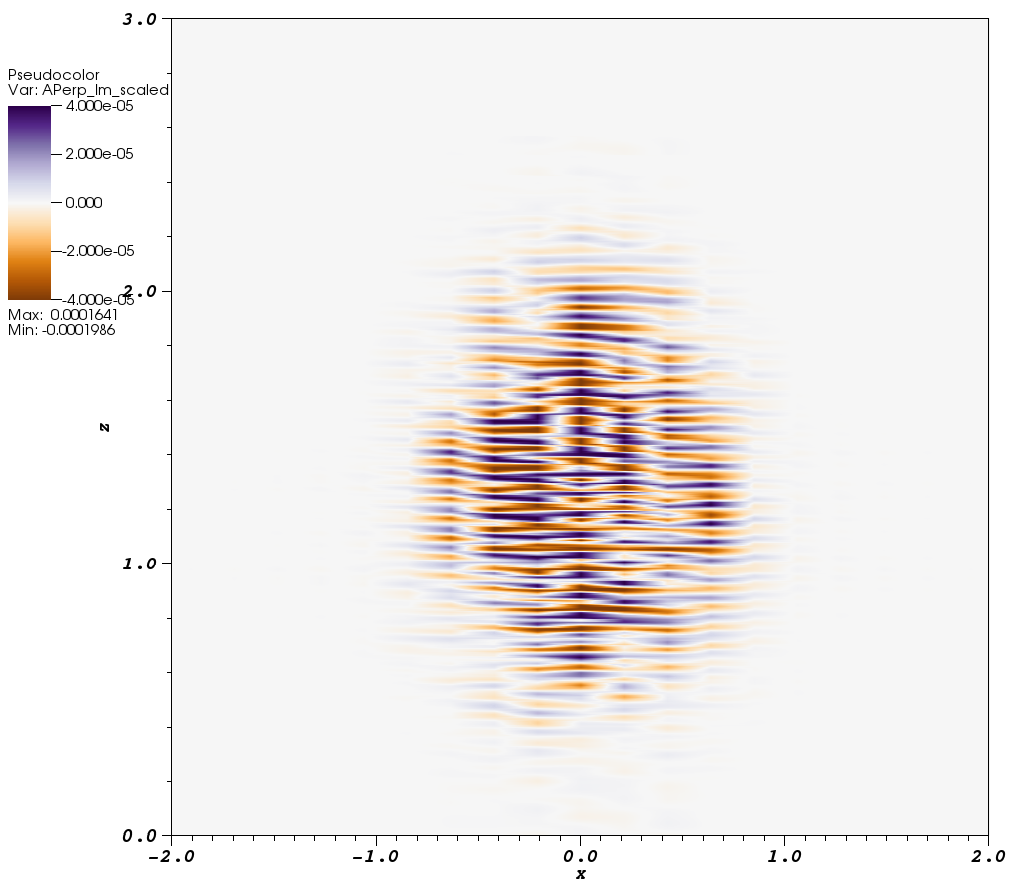
\includegraphics[width=60mm]{visit0032.png}
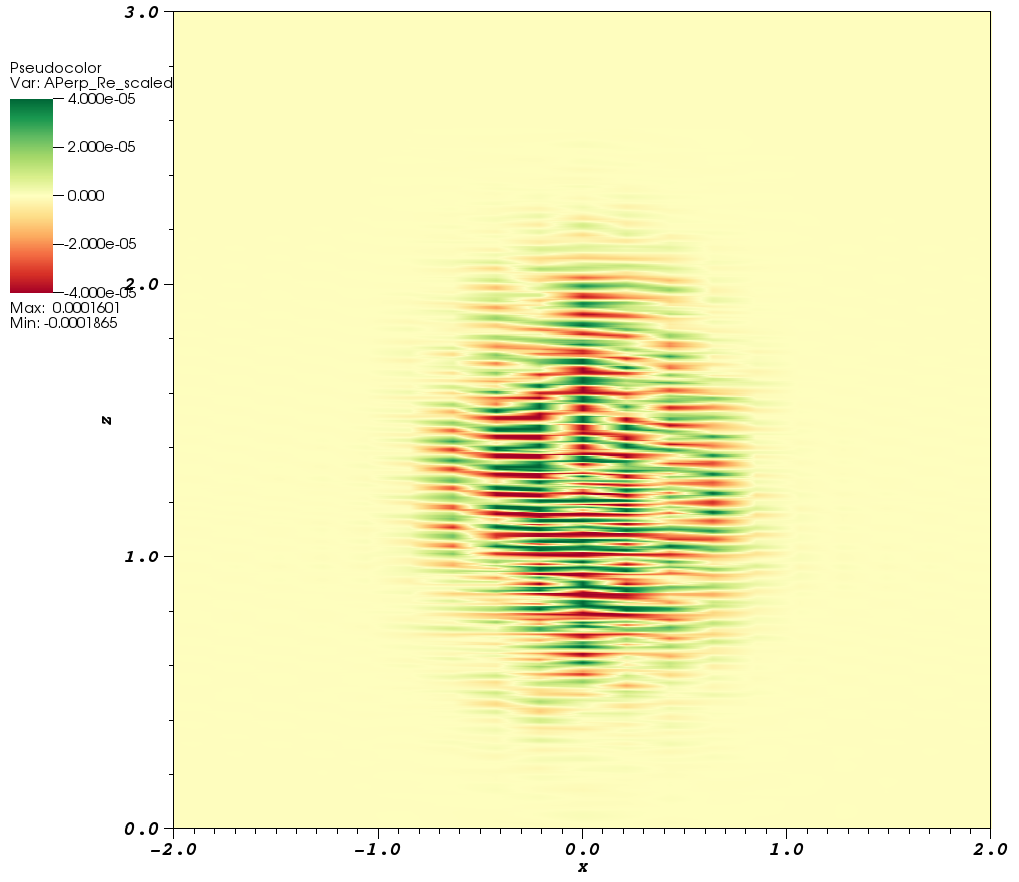
\includegraphics[width=60mm]{visit0033.png}
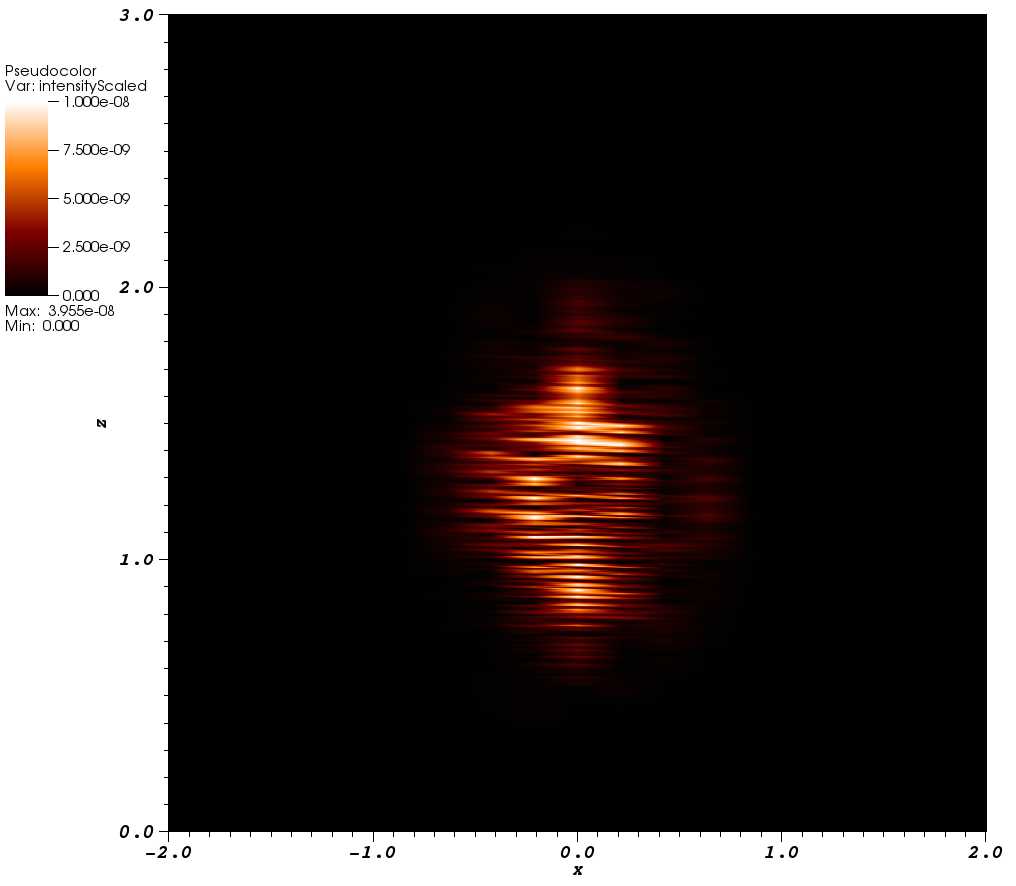
\includegraphics[width=100mm]{visit0035.png}
\caption{Radiated spontaneous field from Puffin in the first few undulator periods - $x$ (top left) and $y$ (top right) polarized fields, and instantaneous intensity (bottom), at $y=0$. Radiation is propagating in the negative $z$ direction (the vertical axis). One can see the noisy phase of the radiation in both transverse (x) and temporal (z) directions, which is due to the shot-noise of the electron beam.  }
\label{bbd1}
\end{figure*}




\begin{figure*}
\centering
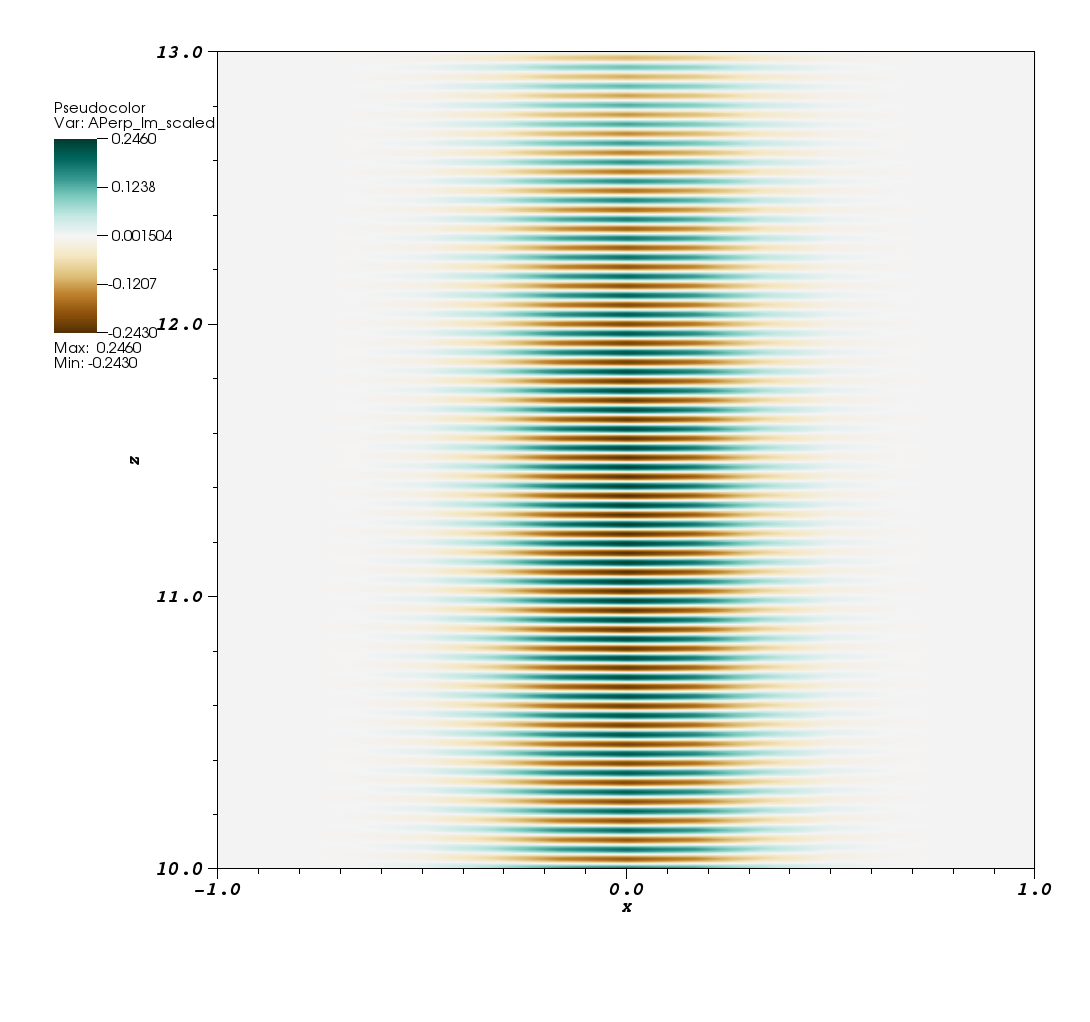
\includegraphics[width=100mm]{visit0036.png}
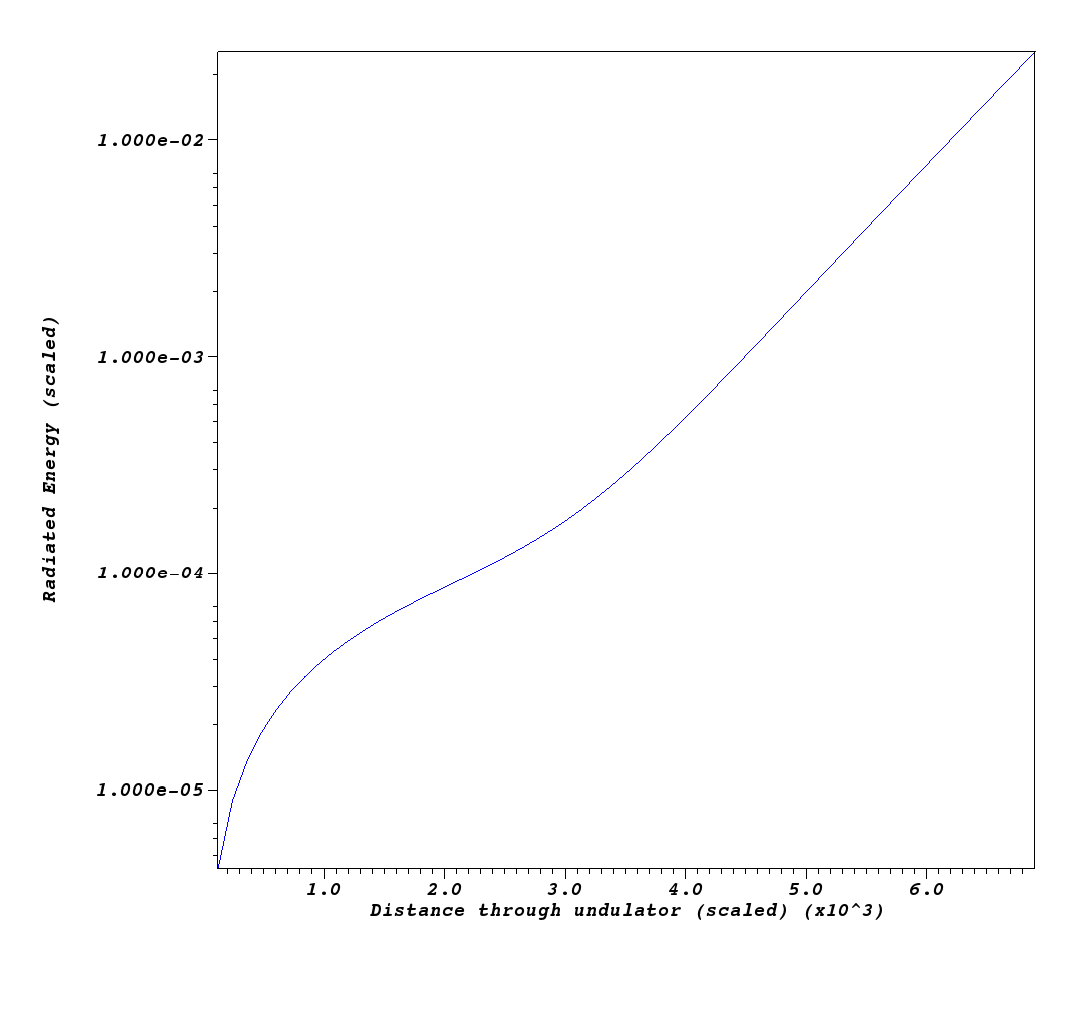
\includegraphics[width=100mm]{visit0037.png}
\caption{Radiated field from Puffin after amplification in the undulator - x polarized field (top). Radiated energy vs scaled distance through the undulator is on the bottom. Observe the noise from the previous figure has disappeared; the amplification process cause the electrons to align and radiate in phase.  }
\label{bbd2}
\end{figure*}

\newpage

\section{Overview}

The system of equations solved by Puffin have been altered from those described in \cite{puffin}. They are now:
\begin{align}
\Bigl[\frac{1}{2}\Bigl(\frac{\partial^2}{\partial\bar{x}^2} + \frac{\partial^2}{\partial\bar{y}^2}\Bigr) -  \frac{\partial^2}{\partial\bar{z}\partial\bar{z}_2}\Bigr]A_{\bot}  & = -\frac{1}{\bar{n}_p}\frac{\partial}{\partial \bar{z}_2}\sum_{j=1}^{N} \frac{\bar{p}_{\bot j}}{\Gamma_j} (1+\eta p_{2j})     \delta^3(\bar{x}_j,\bar{y}_j,\bar{z}_{2j})  \label{fieldeq2} \\
\frac{d \bar{p}_{\bot j}}{d \bar{z}} = & \frac{1}{2\rho}\Bigl[ i \alpha b_{\bot} - \frac{\eta p_{2j}}{\kappa^2}A_{\bot} \Bigr] - i\kappa \frac{ \bar{p}_{\bot j}}{\Gamma_j} (1 + \eta p_{2j})  \alpha b_z \label{pperpeqn2} \\
\frac{d \Gamma_{j}}{d \bar{z}} &= - \rho \frac{(1 + \eta p_{2j})}{\Gamma_j} (\bar{p}_{\bot j} A^*_{\bot j} + c.c.)  \label{gameqn} \\
\frac{d\bar{z}_{2j}}{d\bar{z}}& = p_{2j}  \label{z2eqgen2} \\
\frac{d\bar{x}_j}{d\bar{z}} &=  \frac{2 \rho \kappa}{\sqrt{\eta} \Gamma_j} (1 + \eta p_{2j}) \Re(\bar{p}_{\bot j}) \label{xeqgen2} \\
\frac{d\bar{y}_j}{d\bar{z}} &= - \frac{2 \rho \kappa}{\sqrt{\eta} \Gamma_j}  (1 + \eta p_{2j}) \Im(\bar{p}_{\bot j}). \label{yeqgen2}
\end{align}
%where $\kappa = \dfrac{a_u}{2 \rho \gamma_r}$, which is actually the scaled natural focussing wavenumber $\kappa = \sqrt{2} \bar{k}_\beta$. 



Scaled parameters are:-


%\begin{align}
%\eta = \frac{\lambda_r}{\lambda_w} = \frac{k_w}{k_r}
%\end{align}




\begin{align}
\bar{z}_{2j} &= \frac{ct_j - z}{l_c}, &\bar{z} &= \frac{z}{l_g}, \nonumber \\
\bar{p}_{\bot} &= \frac{p_{\bot}}{mc a_u},
&A_{\bot}&=\frac{e \kappa l_g}{\gamma_0 mc^2 }E_{\bot}, \nonumber \\
(\bar{x},\bar{y}) &= \frac{(x,y)}{\sqrt{l_g l_c}}, &l_g &= \frac{\lambda_w}{4\pi\rho}, \nonumber \\
l_c &= \frac{\lambda_r}{4\pi\rho}, & \Gamma_j& = \frac{\gamma_j}{\gamma_0}, \nonumber \\
\rho &=\frac{1}{\gamma_0}\left(\frac{a_u \omega_p}{4ck_u}\right)^{2/3}, 
&a_u & =\frac{eB_0}{mck_u}, \nonumber \\
\kappa & = \frac{a_u}{2 \rho \gamma_0}, & b_{\bot} & = b_x - i b_y, \nonumber
\end{align}

$B_0$ is the peak magnetic field in the wiggler.
$\omega_p = \sqrt{e^2 n_p / \epsilon_0 m}$ is the (non-relativistic) plasma frequency, and $n_p$ is the peak spatial number density of the electron beam $(N_e / \delta_x \delta_y \delta_z)$. 
$E_\bot = E_x - i E_y$ are the $x$ and $y$ radiation electric field vectors. $\gamma_0$ is the reference energy (Lorentz factor), which is usually taken as the mean beam energy.

The scaled reference velocity, 
\begin{align}
\eta = \frac{1 - \beta_{zr}}{\beta_{zr}} = \frac{\lambda_r}{\lambda_u} = \frac{l_c}{l_g},
\end{align}
where $\beta_{zr}$ is some reference velocity scaled to $c$, which is sensible (but not, strictly speaking, necessary) to take as the mean longitudinal electron velocity in the wiggler, so that
\begin{align}
\beta_{zr} = \sqrt{ 1 - \frac{1}{\gamma_0^2}\Bigl(1 + \bar{a}_u^2\Bigr)},
\end{align}
where $\bar{a}_u$ is the $rms$ undulator parameter.
This defines the velocity at which the electrons travel in the scaled $\bar{z}_2$ frame. More generally, $\eta$ describes an *ideal* resonance condition - electrons resonant with wavelength $\lambda_r$ will travel with velocity $p_2=1$ through the $\bar{z}_2$ frame. 




$p_{2j}$ may be worked out analytically from 
\begin{align}
p_{2j} = \frac{1}{\eta}\Bigl[ \Bigl(  1 - \frac{(1 + a_u^2 | \bar{p}_{\bot j} |^2)}{\gamma_r^2 \Gamma^2_j}  \Bigr)^{-1/2} - 1   \Bigr]
\end{align}
at each step. It is NOT output from Puffin.

Outputs from Puffin are the scaled radiation field $A_\bot$, electron phase space coords $\bar{x}, \bar{y}, \bar{z}_2, \bar{p}_\bot, \Gamma$, and scaled distance through the undulator $\bar{z}$. The normalized electron weights are in the file NormChiDataFile.dat (normalised to the peak *spatial* (3D) density).



Compared to the original Puffin paper \cite{puffin}, now the peak magnetic fields are used to scale the system of eqns (as opposed to the $rms$ values used previously). Previously (\textit e.g. as described in \cite{puffin}), the energy exchange was modelled through the scaled longitudinal velocity $p_2$. This was problematic in multiple ways from a computational point of view, since $p_2$ is a function of the energy, $p_x$ and $p_y$, so that the same quantity was essentially being calculated twice, leading to large errors in some cases. The energy exchange is instead now modelled directly through the scaled variable $\Gamma_j = \gamma_j / \gamma_r$, meaning smaller numerical errors and enabling a significantly larger step size. 

The formalism for including a variation in the magnetic undulator field, so that $B_0(\bar{z})$ now varies, was included in \cite{2col}, and is varied using the parameter $\alpha(\bar{z}) = \dfrac{B_0(\bar{z})}{B_0(\bar{z}=0)}$.

In the most basic form, the input requires 3 files - a `main' input file for parameters, numerical integration, and description of the field mesh, a `beam' input file descibing the electron beam, and a `seed' input file describing the radiation seed. Optionally, a lattice file can be used to setup an undulator-chicane lattice.

\subsection{Parameters}

Description of parameters:-

{\bf sRho}

$\rho$, the FEL parameter. This specifies the scaling of the system. It does {\bf not} have to be strictly correct - it only descibes the scaling. The simulation can be performed, and the system may be scaled back to SI units using the supplied scripts (NOT SUPPLIED YET!!). If it is correct, however (meaning, it has been calculated from the beam and undulator parameters input), then the scaled notation becomes physically relevant. For an ideal, 1D system, the system should saturate at intensity $|A|^2 \approx 1$, and the system should be firmly in the high or exponential gain regime at $\bar{z} \approx 2-3$. This allows one to see how efficiently the system is lasing w.r.t its ideal case.


{\bf saw}

$a_u$, the undulator parameter defined with the peak on-axis magnetic field.

{\bf sgamma\_r}

$\gamma_0$, the reference (usually the mean) beam energy.

{\bf lambda\_w}

$\lambda_u$, the undulator, or wiggler, period.

{\bf zundType}

Allows one to select from a choice of undulators. Choices are `curved', `planepole', and `helical', described analytically below. If neither of these are chosen, then the default elliptical undulator is chosen, with polarization specified by $u_x$ and $u_y$.

{\bf sux, suy}

$u_x$ and $u_y$ - the relative peak magnetic field of the undulator in each transverse polarization. Usually, at least one should be $=1$, and the other between $0$ (planar) and $1$ (helical). If they are not defined, the default is helical, $u_x=u_y=1$.


{\bf qOneD}

Logical. If  {\bf .true.}, Puffin will be run in 1D mode. Default is  {\bf .true.}, since this is the least computationally expensive option.

{\bf qFieldEvolve}

Logical. If = {\bf .false.}, then the radiation field evolution will be switched off. This is obviously artificial and very rarely used, but can be useful for debugging in some instances. Default is = {\bf .true}.

{\bf qElectronsEvolve}

Logical. If = {\bf .false.}, then the electron equations are not solved in the integration steps. Like when qFieldEvolve= {\bf .false.},  this is obviously artificial and very rarely used, but can be useful for debugging in some instances. Default is = {\bf .true.}.

{\bf qElectronFieldCoupling}

Logical. If = {\bf .false.}, then the radiation field feedback onto the electrons is switched off by setting the field terms in the electron evolution equations = 0, and so switches off the amplification of the radiation from the electrons. This is unphysical, but is used more often than when qFieldEvolve and qElectronsEvolve ={\bf .false.} . It can often be used to check for gain in the FEL in low gain situations, or to check whether amplification has occurred rather than coherent emission (CSE) effects due to \textit{e.g.} fine structure in the beam. When ={\bf .false.}, this will give the purely spontaneous emission (coherent or incoherent) from the electrons in the wiggler. If there is no appreciable difference between the qElectronFieldCoupling=true and false cases, then there has been negligible FEL amplification.

{\bf qFocussing}

Allows one to switch the strong focussing channel on or off. If ={bf .true.}, the strong focusing is switched on with calues specified by sKBetaXSF and sKBetaYSF. If qFocussing={\bf .true.}, yet no focussing strength is specified (sKBetaXSF or sKBetaYSF), then strong focusing is effectively switched off in that dimension. Default = {\bf .false.}.

{\bf qDiffraction}

Switches modelling of diffraction of the radiation field on or off. If ={\bf .true.}, field diffraction is modelled. This can be useful to switch off only really for debugging purposes. Default ={\bf .true.}.



\subsection{3D Magnetic Fields}

The undulator is modelled analytically, and the model must include the fast wiggle motion. Puffin may be modified in the future to allow a map of the undulator field to be input. For now, there are a few generic undulator model employed. The magnetic fields for use in Puffin are the helical, plane-pole, and canted-pole undulator fields discussed in \cite{scharlemann1}, which in the scaled notation here are:-

{\bf helical}
\begin{align}
b_x  & = \cos({\bar{z}/2\rho}) \\
b_y & =  \sin({\bar{z}/2\rho}) \\
b_z & = \frac{\sqrt{\eta}}{2\rho} (-\bar{x}\sin({\bar{z} / (2 \rho)}) + \bar{y}\cos({\bar{z} / (2 \rho)}))
\end{align}


{\bf plane-pole}
\begin{align}
b_x  & = 0 \\
b_y & =  \cosh((\sqrt{\eta}/{2\rho}) \bar{y}) \sin({\bar{z}/2\rho}) \\
b_z & =   \sinh((\sqrt{\eta}/{2\rho}) \bar{y}) \cos({\bar{z} / (2 \rho)}
\end{align}




{\bf canted-pole}
\begin{align}
b_x  & =  \frac{\bar{k}_{\beta x}}{\bar{k}_{\beta y}}  \sinh(\bar{k}_{\beta x} \bar{x} )  \sinh(   \bar{k}_{\beta y} \bar{y}    )   \sin({\bar{z}/2\rho}) \label{cp1} \\
b_y & =   \cosh(\bar{k}_{\beta x} \bar{x} )  \cosh(   \bar{k}_{\beta y} \bar{y}    )   \sin({\bar{z}/2\rho}) \label{cp2}\\
b_z & = \frac{\sqrt{\eta}}{2\rho \bar{k}_{\beta x}}     \cosh(\bar{k}_{\beta x} \bar{x} )    \sinh(   \bar{k}_{\beta y} \bar{y}    )    \cos({\bar{z}/2\rho}) \label{cp3}
\end{align}


{\bf variably polarized elliptical}
\begin{align}
b_x  & = u_x \cos({\bar{z}/2\rho}) \\
b_y & =  u_y \sin({\bar{z}/2\rho}) \\
b_z & = \frac{\sqrt{\eta}}{2\rho} (u_x \bar{x}\sin({\bar{z} / (2 \rho)}) + u_y \bar{y}\cos({\bar{z} / (2 \rho)}))
\end{align}


In the $1$D approximation, $b_z = 0$. 

All of the above have an associated `natural' focusing channel, which arises from from the off-axis variation in the magnetic fields. This motion arises naturally when numerically solving the equations, and is not super-imposed upon the electron motion. 

\subsection{Undulator Ends}

The undulators also include entry and exit tapers, and they may be switched on or off in the input file with the flag {\bf qUndEnds}. Setting this to true will model a smooth taper up and down of the undulator magnetic fields in the first and last 2 periods of the undulator, taking the form of a $\cos^2$. If they are switched off, the beam is artificially initialized with an `expected' initial condition in the transverse coordinates for that undulator. Including these ends will model a more realistic and natural entry and exit from the undulator, and will reduce CSE effects from the shape of the wiggler.

The precise description of the undulator ends are as follows. Note the presence of corrective terms in addition to the main $\cos^2$ term, which ensure the beam oscillates close to the axis. (Note also the very small non-zero initial $z-$magnetic field in each case, which we find  has no noticable deleterious effects in practice.)

{\bf Helical Front}

\begin{align}
b_x  =  \frac{1}{4}\sin(\bar{z}/16\rho) & \cos(\bar{z}/16\rho)    \sin(\bar{z}/2\rho)   +   \sin^2(\bar{z} / 16\rho)  \cos(\bar{z}/2\rho)  \\  
b_y =  - \frac{1}{4}\sin(\bar{z}/16\rho) & \cos(\bar{z}/16\rho)    \cos(\bar{z}/2\rho)   +  \sin^2(\bar{z} / 16\rho)  \sin(\bar{z}/2\rho)\\
b_z = \frac{\sqrt{\eta}}{2\rho} \Bigl[   \bar{x}\Bigl(& \frac{1}{32}\cos( \bar{z}/8\rho )\sin(\bar{z}/2\rho) +
           \frac{1}{4}\sin(\bar{z}/8\rho)\cos(\bar{z}/2\rho) \nonumber  \\
           & - \sin^2(\bar{z}/16\rho)\sin(\bar{z}/2\rho) \Bigr) \nonumber \\
           \bar{y}\Bigl(& -\frac{1}{32}\cos( \bar{z}/8\rho )\cos(\bar{z}/2\rho) +\frac{1}{4}\sin(\bar{z}/8\rho)\sin(\bar{z}/2\rho) \nonumber  \\
           & + \sin^2(\bar{z}/16\rho)\cos(\bar{z}/2\rho) \Bigr)  \Bigr]  
\end{align}


{\bf Helical Back}

\begin{align}
b_x  =  -\frac{1}{4}\cos(\bar{z}/16\rho) & \sin(\bar{z}/16\rho)    \sin(\bar{z}/2\rho)   +   \cos^2(\bar{z} / 16\rho)  \cos(\bar{z}/2\rho)  \\
b_y =  \frac{1}{4}\cos(\bar{z}/16\rho) & \sin(\bar{z}/16\rho)    \cos(\bar{z}/2\rho)   +  \cos^2(\bar{z} / 16\rho)  \sin(\bar{z}/2\rho)\\
b_z = \frac{\sqrt{\eta}}{2\rho} \Bigl[   \bar{x}\Bigl(& -\frac{1}{32}\cos( \bar{z}/8\rho )\sin(\bar{z}/2\rho) -
           \frac{1}{4}\sin(\bar{z}/8\rho)\cos(\bar{z}/2\rho) \nonumber  \\
           & - \cos^2(\bar{z}/16\rho)\sin(\bar{z}/2\rho) \Bigr) \nonumber \\
           \bar{y}\Bigl(& \frac{1}{32}\cos( \bar{z}/8\rho )\cos(\bar{z}/2\rho) - \frac{1}{4}\sin(\bar{z}/8\rho)\sin(\bar{z}/2\rho) \nonumber  \\
           & + \cos^2(\bar{z}/16\rho)\cos(\bar{z}/2\rho) \Bigr)  \Bigr] 
\end{align}



{\bf Plane-Pole Front}

\begin{align}
b_x  =  0,  &    \\
b_y   = \cosh(\sqrt{\eta}\bar{y} / 2\rho)\Bigl[ -\frac{1}{4}& \sin(\bar{z}/16\rho) \cos(\bar{z}/16\rho) \cos(\bar{z} / 2\rho) +   \sin^2(\bar{z}/16\rho) \sin(\bar{z} / 2\rho)   \Bigr], \\
b_z  =  \sinh(\sqrt{\eta}\bar{y} / 2\rho) \Bigl[ -\frac{1}{32} & \cos(\bar{z}/8\rho) \cos(\bar{z}/2\rho) + \nonumber \\ 
                                                &\frac{1}{4}  \sin(\bar{z}/8\rho)\sin(\bar{z}/2\rho) + \sin^2  (\bar{z}/16\rho) \cos(\bar{z}/2\rho)  \Bigr],
\end{align}

{\bf Plane-Pole Back}

\begin{align}
b_x  =  0,  &    \\
b_y   = \cosh(\sqrt{\eta}\bar{y} / 2\rho)\Bigl[ \frac{1}{4}& \sin(\bar{z}/16\rho) \cos(\bar{z}/16\rho) \cos(\bar{z} / 2\rho) +   \cos^2(\bar{z}/16\rho) \sin(\bar{z} / 2\rho)   \Bigr], \\
b_z  =  \sinh(\sqrt{\eta}\bar{y} / 2\rho) \Bigl[ \frac{1}{32} & \cos(\bar{z}/8\rho) \cos(\bar{z}/2\rho) - \nonumber \\ 
                                                &\frac{1}{4}  \sin(\bar{z}/8\rho)\sin(\bar{z}/2\rho) + \cos^2  (\bar{z}/16\rho) \cos(\bar{z}/2\rho)  \Bigr].
\end{align}



{\bf Curved-Pole Front}


\begin{align}
b_x  =  \frac{\bar{k}_{\beta x}}{\bar{k}_{\beta y}} \sinh(\bar{k}_{\beta x} \bar{x})\sinh(\bar{k}_{\beta y} \bar{y}) \Bigl[ -\frac{1}{8}& \sin(\bar{z}/8\rho) \cos(\bar{z} / 2\rho) +   \sin^2(\bar{z}/16\rho) \sin(\bar{z} / 2\rho)   \Bigr],    &    \\
b_y   =  \cosh(\bar{k}_{\beta x} \bar{x})\cosh(\bar{k}_{\beta y} \bar{y}) \Bigl[ -\frac{1}{8}& \sin(\bar{z}/8\rho) \cos(\bar{z} / 2\rho) +   \sin^2(\bar{z}/16\rho) \sin(\bar{z} / 2\rho)   \Bigr], \\
b_z  =  \frac{\sqrt{\eta}}{2 \rho \bar{k}_{\beta y}}  \cosh(\bar{k}_{\beta x} \bar{x})\sinh(\bar{k}_{\beta y} \bar{y})  \Bigl[ -\frac{1}{32} & \cos(\bar{z}/8\rho) \cos(\bar{z}/2\rho) + \nonumber \\ 
                                                &\frac{1}{4}  \sin(\bar{z}/8\rho)\sin(\bar{z}/2\rho) + \sin^2  (\bar{z}/16\rho) \cos(\bar{z}/2\rho)  \Bigr] .
\end{align}

{\bf Curved-Pole Back}

\begin{align}
b_x  =  \frac{\bar{k}_{\beta x}}{\bar{k}_{\beta y}} \sinh(\bar{k}_{\beta x} \bar{x})\sinh(\bar{k}_{\beta y} \bar{y}) \Bigl[ \frac{1}{8}& \sin(\bar{z}/8\rho) \cos(\bar{z} / 2\rho) +   \cos^2(\bar{z}/16\rho) \sin(\bar{z} / 2\rho)   \Bigr],    &    \\
b_y   =  \cosh(\bar{k}_{\beta x} \bar{x})\cosh(\bar{k}_{\beta y} \bar{y}) \Bigl[ \frac{1}{8}& \sin(\bar{z}/8\rho) \cos(\bar{z} / 2\rho) +   \cos^2(\bar{z}/16\rho) \sin(\bar{z} / 2\rho)   \Bigr], \\
b_z  =  \frac{\sqrt{\eta}}{2 \rho \bar{k}_{\beta y}}  \cosh(\bar{k}_{\beta x} \bar{x})\sinh(\bar{k}_{\beta y} \bar{y})  \Bigl[ \frac{1}{32} & \cos(\bar{z}/8\rho) \cos(\bar{z}/2\rho) - \nonumber \\ 
                                                &\frac{1}{4}  \sin(\bar{z}/8\rho)\sin(\bar{z}/2\rho) + \cos^2  (\bar{z}/16\rho) \cos(\bar{z}/2\rho)  \Bigr] .
\end{align}



\subsection{Natural Undulator Focusing}

Each undulator type has an associated natural focusing wavenumber. In the helical case, the natural betatron wavenumber is
\begin{align}
\bar{k}_{\beta n x} = \bar{k}_{\beta n y} = \frac{a_w}{2 \sqrt{2} \rho \gamma_0},
\end{align}
with $\gamma_0$ being the average beam energy (and not necessarily = $\gamma_r$)

In the planar case,
\begin{align}
\bar{k}_{\beta n y} = \frac{a_w}{2 \sqrt{2} \rho \gamma_0}.
\end{align}

In the canted pole case,
\begin{align}
\bar{k}_{\beta n x,y} = \frac{a_w \bar{k}_{x,y}}{\sqrt{2 \eta} \gamma_0},
\end{align}
where $\bar{k}_{x,y}$ describe the hyperbolic variation in the transverse directions (see eqns (\ref{cp1} - \ref{cp3})), and must obey 
\begin{align}
\bar{k}_x^2 + \bar{k}_y^2 = \frac{\eta}{4 \rho^2}
\end{align}
to be physically valid. They determine the focusing strength in the $\bar{x}$ and $\bar{y}$ dimensions. For the case of equal focusing, then,
\begin{align}
\bar{k}_{\beta n x} = \bar{k}_{\beta n y} = \frac{a_w }{ 4 \rho \gamma_0}.
\end{align}



\subsection{Strong Beam Focusing}

In addition to the natural focusing channel, a constant, `strong' focussing channel may be utilized, to focus the beam to a smaller transverse area. This is a magnetic field super-imposed upon the wiggler. It may be switched on or off with the flag {\bf qFocussing} in the main input file, and is specified through the use of the variables {\bf sKBetaXSF} and {\bf sKBetaYSF}. It is probably highly artificial - it may be thought of as physically similar to an ion channel. Nevertheless it allows one to obtain strong focusing without using a lattice. It is defined very simply as 
\begin{align}
b_x = \sqrt{\eta} \frac{\bar{k}_{\beta y}^2}{\kappa}\bar{y}_j, \\
b_y = - \sqrt{\eta} \frac{\bar{k}_{\beta x}^2}{\kappa}\bar{x}_j
\end{align}

If either {\bf sKBetaXSF} or {\bf sKBetaYSF} are not specified, then no focusing channel will be added for that dimension, even if the {\bf qFocussing} flag is true.

Magnetic quads will be added soon.


\subsection{Auto beam-matching}

The beam, when specified by the `simple' method (see below) may be matched to the focusing channel automatically with the flag {\bf qMatched\_A} in the beam file - the option can be set for each beam. In the scaled notation,
\begin{align}
\bar{\sigma}_{x,y} = \sqrt{  \frac{ \rho \bar{\epsilon}_{x,y} }{\bar{k}_{\beta x,y} }  }
\end{align}
where $\bar{\epsilon}_{x,y} = \epsilon_{x,y} / (\lambda_r / 4\pi)$ are the transverse emittances scaled to the so-called Kim criterion.

%If we define $\bar{a}_w$ as the $rms$ undulator parameter, so that  $\bar{a}_w = a_w$ in the helical case, and  $\bar{a}_w = a_w / sqrt{2}$ in the planar and canted pole case, then we can write a general expression


The spread in the transverse momentum directions is then given by 
\begin{align}
\bar{\sigma}_{px, py} = \frac{\sqrt{\eta}}{2 \kappa} \Bigl<  \frac{\Gamma}{1+\eta p_{2}}  \Bigr> \frac{ \bar{\epsilon}_{x,y} }{\bar{ \sigma}_{x,y}}.   \label{tmtch_spd} 
\end{align}
where angular brackets indicate the ensemble average of the beam.

If {\bf qFocussing} is true and the strong betatron wavenumber is given, then the strong betatron wavenumber is used to match the beam. Otherwise the beam is auto-matched to the natural focusing channel of the undulator. 




\subsection{To scale or not to scale?}

The main algorithm in Puffin utilizes scaled variables to make the numbers `nicer' to work with. The system saturates with scaled intensity $\sim 1$, the scaled perpindicular momentum of the beam in the wiggler oscillates between $-1$ and $1$, and so forth. The distance through the wiggler is given in units of a (1D) gain length, and the beam coordinate in the radiation frame is in units of the cooperation length, so that an electron slips $1l_c$ through the radiation field in $1$ gain  length. The scaling defines a frame of reference which normalises the quantities not only to numerically more manageable numbers, but to \textit{characteristic} variables. 

The two dominant variables for the scaling are $\rho$ and $\eta$. $\eta$ is a function of the wiggler parameters $a_u$ and $\lambda_u$, and reference beam energy $\gamma_r$, and is calculated in Puffin from the input. The $\rho$ parameter is dependent on the peak electron beam number density, amongst other things.

The beam and radiation field parameters may be input in either SI units or the scaled units. Use the variable {\bf qscaled} in the main input file to do this. If $=$ {\bf .true.}, then Puffin expects scaled variables are being used. If SI units are used, then the input parameters will be scaled according to the scaling values specified in the main input file. 

Note that they are only \textit{scaling} parameters. The FEL parameter as input does not have to correspond to the beam being input for the results to be correct. The scaled parameters will behave `nicely' if it does, but it is not necessary. When the result is unscaled, the resut will still be correct.



\begin{table}
\centering
\caption[Input Units]{Input Dimensions and Units for Beam and Radiation Field}
\begin{tabular}{|  c   | c  |   c   |}
\hline
Unscaled & units & unscaled equivalent \\
\hline
$x$ & metres (m) & $\bar{x}$ \\
\hline
$y$ & metres (m) & $\bar{y}$ \\
\hline
$dx/dz$ & dimensionless & $\bar{p}_x$ \\
\hline
$dy/dz$ & dimensionless & $\bar{p}_y$ \\
\hline
$t$ & seconds (s) & $\bar{z}_2$ \\
\hline
\end{tabular}
\label{table}
\vspace*{-\baselineskip}
\end{table}



%%% Beam energy - what is the unscaled input?
%%% Have to explain the 'mean' beam energy and 
%%% the rms width in energy are in what units...??










\subsection{Beam Initialization}

There are 3 different ways of defining and initializing the electron beam in Puffin:

\subsubsection{Simple}

The beam is described in terms of a homogeneous Gaussian function in every dimension. Some simple correlations in energy can be achieved by specifying an oscillation in the beam energy as a function of $\bar{z}_2$, or as a simple linear energy chirp in $\bar{z}_2$. The beam is generated in Puffin according to this description.

In general, the correct noise statistics are added to the beam with the method described in REF (see figure REF). This method, like other noise algorithms, requires a quiet beam to add the noise to. We include two methods of generating the beam - one with the correct noise in all dimensions, and one with the correct noise only in the temporal/$\bar{z}_2$ dimension. In both methods, the beam is initially quiet in the temporal dimension before adding the noise, with an equispaced layout of the particles in this dimension. The beam MUST be created to appropriately sample the wavelength of emission/amplification - so at least 10 equispaced particles per resonant wavelength. The methods are:-

% qSI - input in SI units - so x, y, z, px, py and gamma - system is then scaled to rho
% Rho and charge are decoupled - so the simulation will always be correct. For the scaled notation to make sense, the rho must be approximately correct for the given beam charge.
% qEqui = .false. by default.



{\bf Equispaced Grid in Every Dimension}

When using this option, the beam is intialized on an equispaced 6D grid. This requires very many particles to appropriately sample every dimension, and you may find it very easy to have more macroparticles than real electrons while loading the beam this way. However, we leave it up to the user to decide if this is appropriate - for some extreme dispersion situation with high charge it may be necessary to create the beam in this way.  This can be activated by setting qEquiXY $=$ true in the beam input. qEquiXY is actually an array of size nbeams, with a seperate value for each beam if multiple beams are desired. qEquiXY $=$ false by default.

{\bf Equispaced grid ONLY in $\bar{z}_2$}

If qEquiXY is false, then the beam is intially generated as a 1D beam, with equispaced macroparticles. Each macroparticle is then split into many particles in the other 5 dimensions, with coordinates generated by a quasi-random sequence in each dimension. The SAME SEQUENCE is used for each particle in z2 - the creates a series of beamlets in the $\bar{z}_2$ dimension, giving a quiet start in $\bar{z}_2$. Because random sequences are used, the other 5-dimensions require orders of magnitude less particles to adequately fill the phase space than in the equispaced case. This is the default option, so if not specified, qEquiXY $=$ false. 

Both of the above methods may, of course, be replicated and modified by the user to suit a particular situation. The creation of the beam with the correct statistics, while still retaining the sampling necessary for the FEL interaction, is still an area of ongoing research, and is quite controversial. We ultimately leave it to the user to ensure the beam is appropriately initialized for their situation. The methods above can probably be replicated with just a few lines of \textit{e.g.} Python. The generated beam can then be input into Puffin.

To use this, set the option dtype = `simple' in the nblist namelist in the beam file. The parameters for the distribution are then set in the blist namelist in the same file.

\subsubsection{Dist input}

The input is composed of a description of temporal slices along the bunch, describing a Gaussian mean and standard deviation in every other dimension for each temporal slice. This information is used to generate the electron beam in Puffin.

\subsubsection{Beam input}

This method allows one to read in the 6D scaled particle coordinates from a text file. The beam is generated externally. (Arrangement?) The user is then responsible for the noise in the pulse - it is not added by Puffin in this method.


\subsection{Field Mesh}


The radiation field in Puffin is modelled by a simple cartesian mesh, with equispaced nodes in each of the 3 spatial dimensions. Each node samples a value of the $x$ and $y$ polarized radiation field (the $z$ component of the electric field is not modelled). The scaled $\bar{z}_2$ coordinate frame is such that the back of the system is with increasing $\bar{z}_2$ - \textit{i.e.} to the right in figure \ref{lgmsh}. Recall that $\bar{z}_2$ is the stationary radiation frame, so that as the beam propagates through the undulator, the beam slips back through the radiation field, moving to the right in figure \ref{lgmsh}. 

This mesh must be large enough to contain the beam through the entire propagation distance through the wiggler.

It must also be large enough to contain the beam in the transverse plane, see figure \ref{trmsh}. The radiation field is calculated from the driving electron beam by linear interpolants, so the field must adequately sample the area which the beam occupies.  The radiation also diffracts outwards from the beam, so the field mesh must extend to adequately model this diffracting radiation to avoid numerical problems at the boundaries of the grid. There are absorbing boundaries in the outer 16 nodes in the mesh in $x$ and $y$ to mitigate this issue, but an absorbing boundary which works well for the full range of frequencies modelled by Puffin is difficult to realise, and the absorbing boundary should not be relied upon to absorb everything which propagates to the outer reaches of the mesh.

\subsection{Fixing the Radiation Mesh}

One may use the variables {\bf iRedNodesX, iRedNodesY} to fix the mesh around the beam - see figure \ref{trmsh}. These variables define an inner set (`reduced' set) of nodes which the beam width will occupy. So the mesh length in $x$ and $y$ will be set up such that the inner set of nodes defined by  {\bf iRedNodesX, iRedNodesY} will contain the beam. In this case, the {\bf sFModelLengthX, sFModelLengthX} inputs will be ignored.


\begin{figure*}
\centering
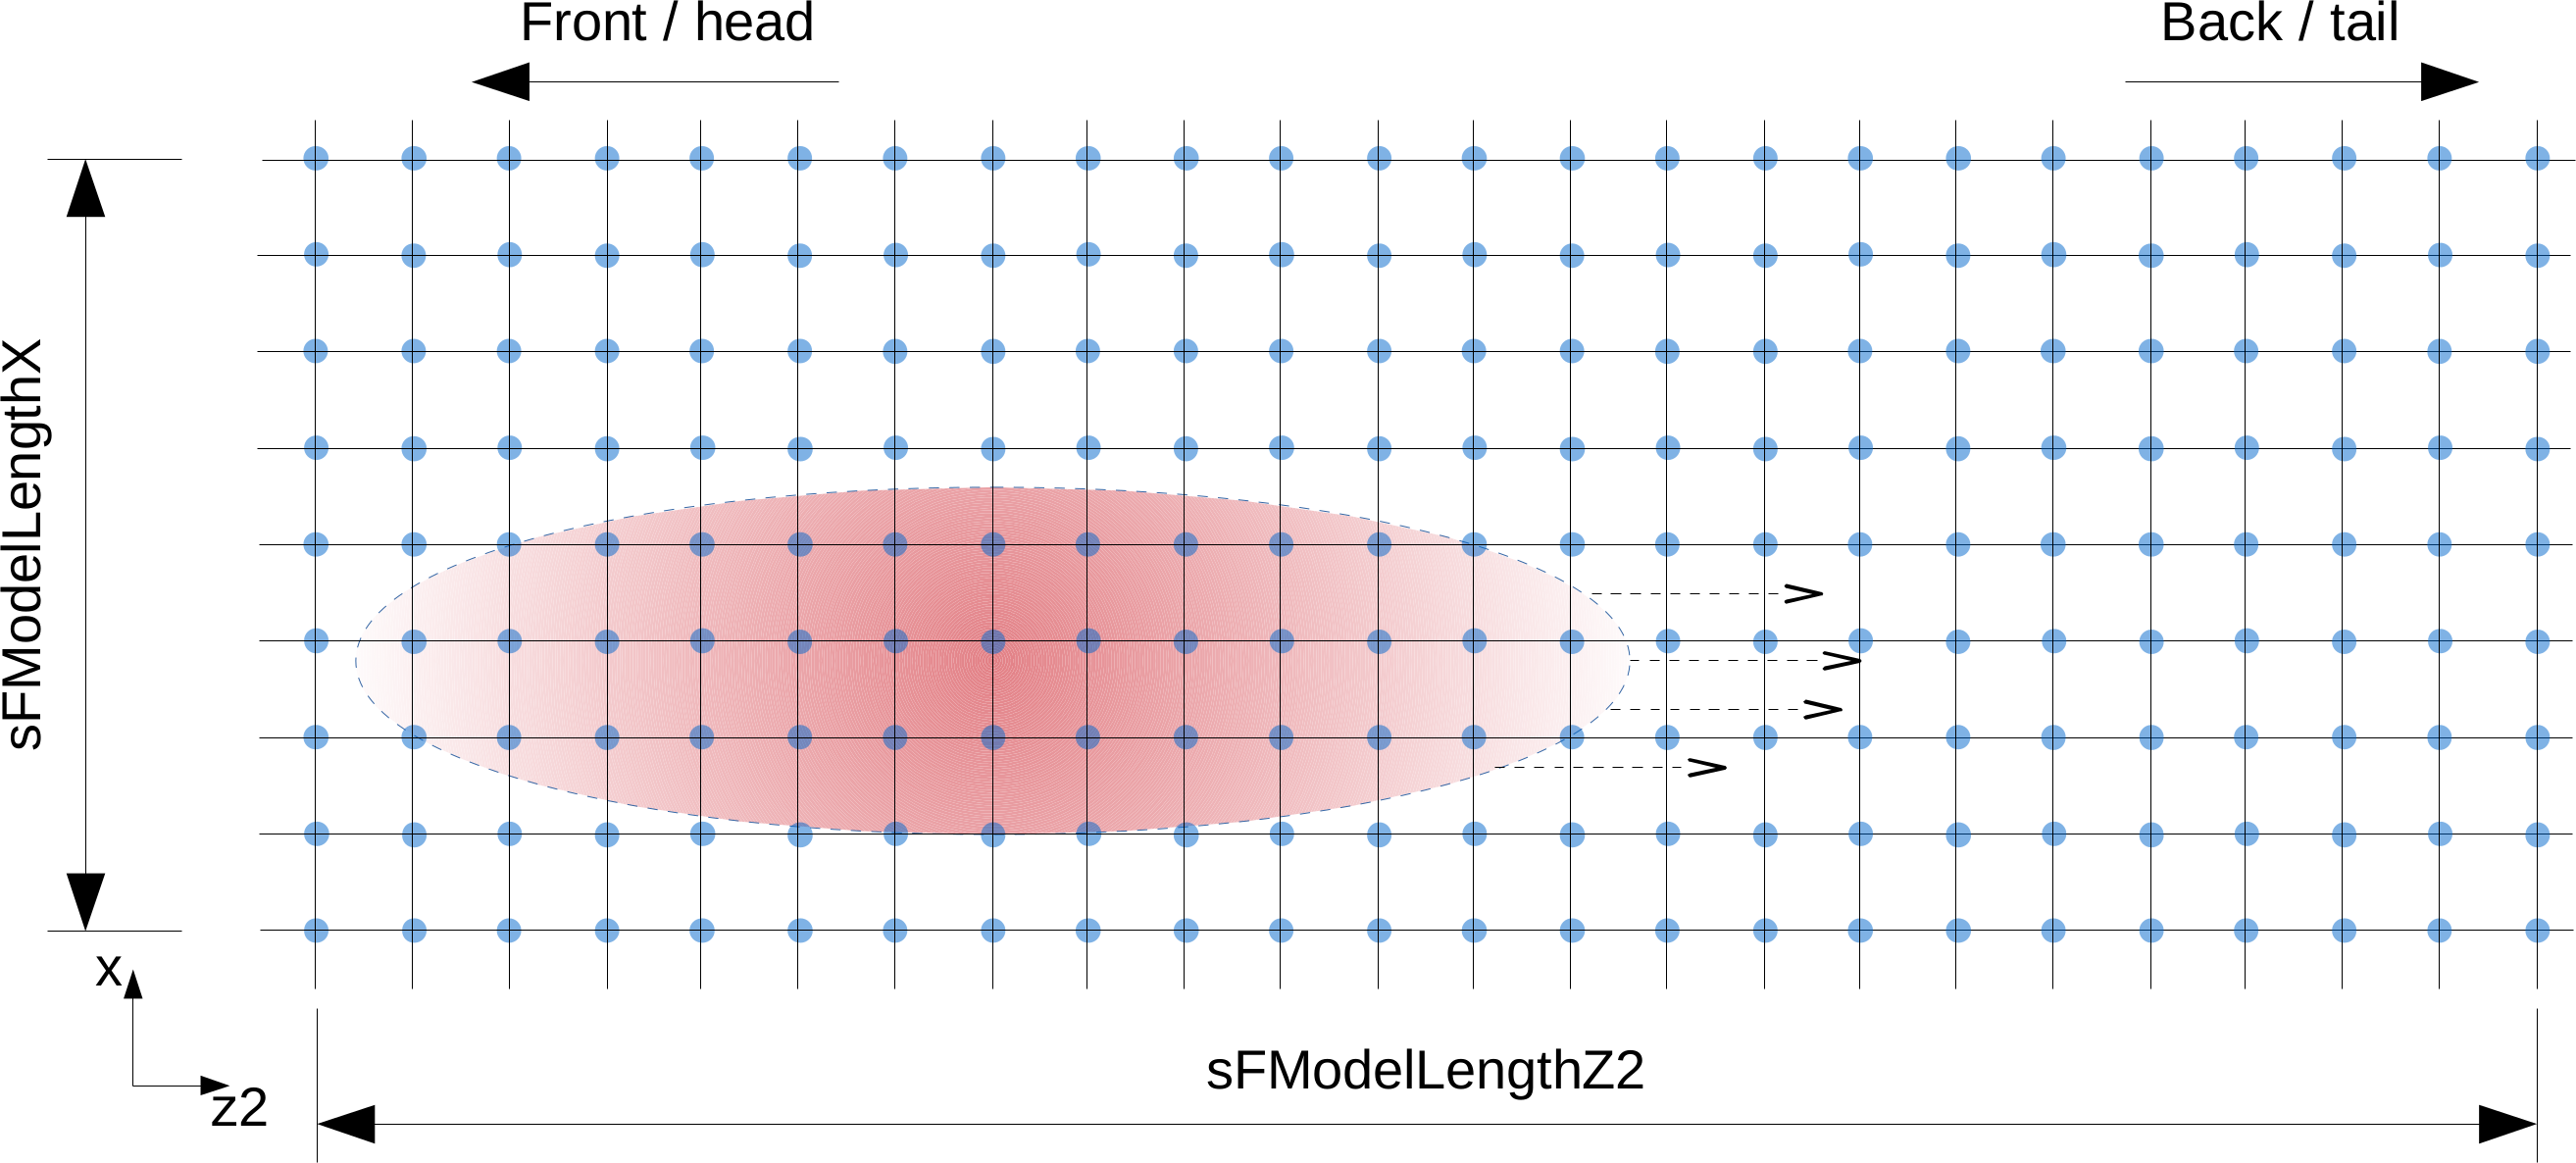
\includegraphics[width=150mm]{long_mesh.png}
\caption{Showing the longitudinal setup of the radiation mesh. The beam is indicated in red. The scaled $\bar{z}_2$ coordinate is defined so that the front of the radiation and beam is to the left. This is the constant radiatioon frame, so the beam slips backwards through the field from left to right. In the lab frame, the beam and radiation propagates from right to left. The full length of the mesh must be large enough to contain the beam through propagation.}
\label{lgmsh}
\end{figure*}


\begin{figure*}
\centering
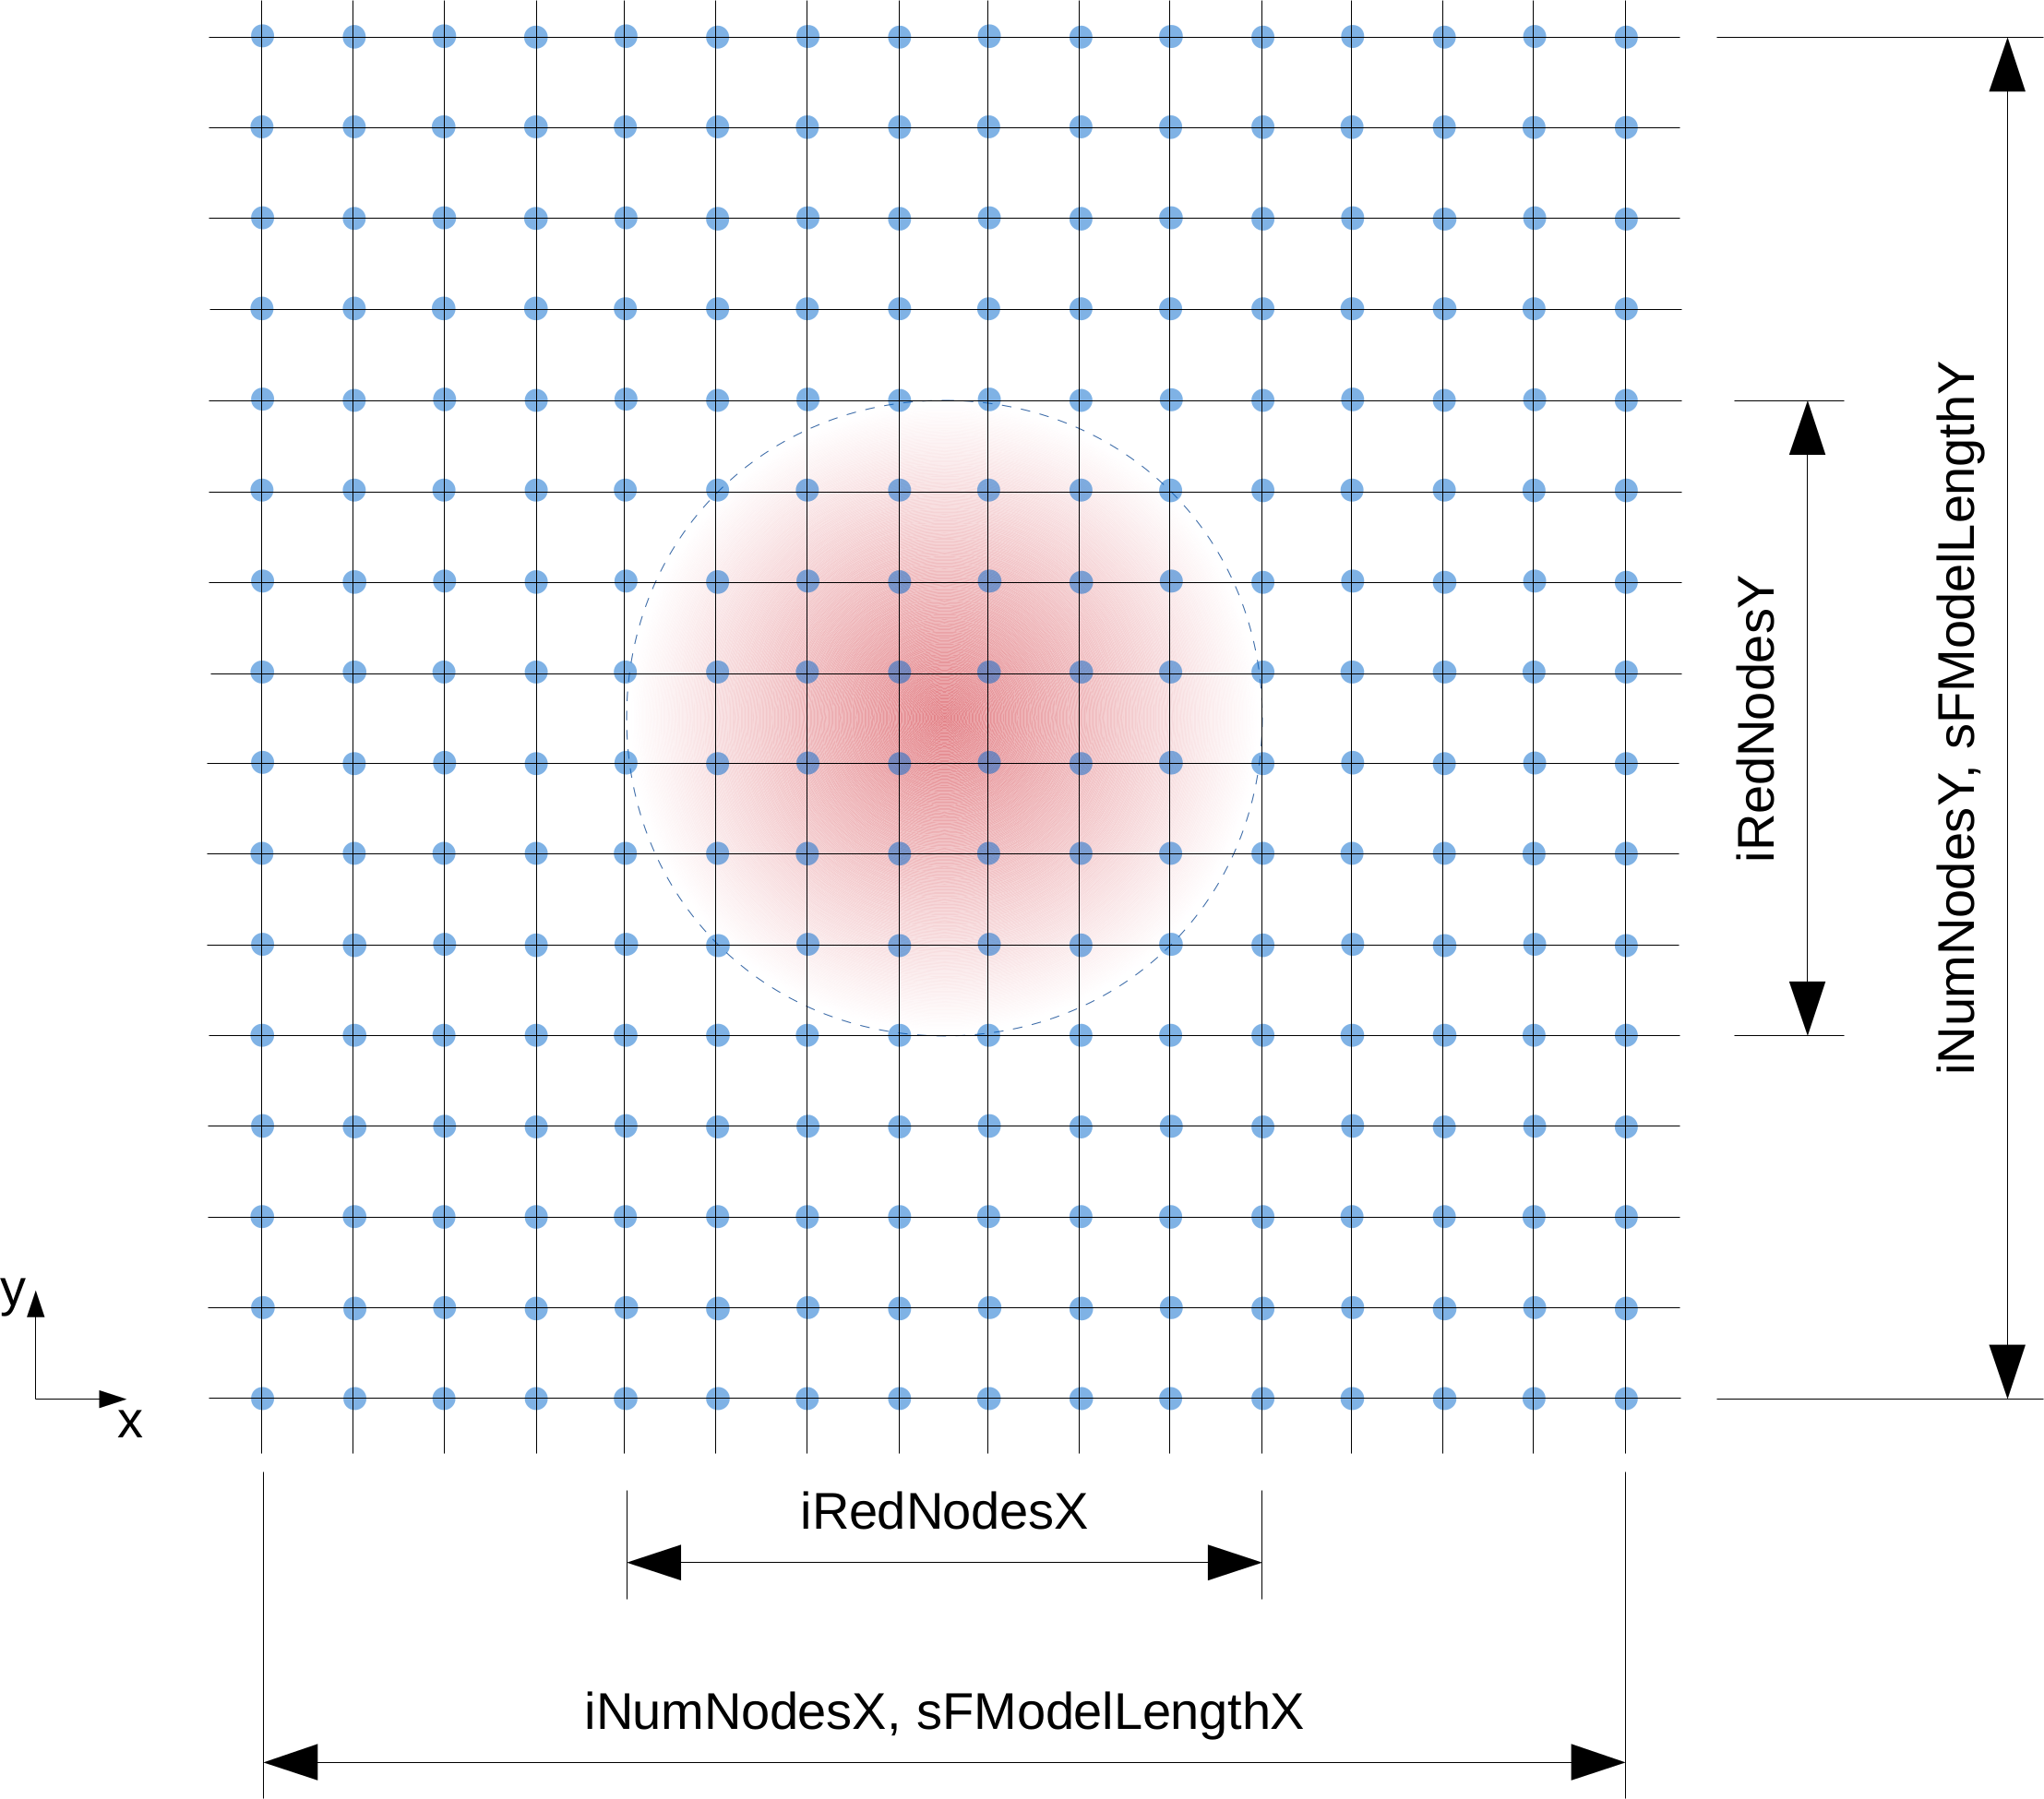
\includegraphics[width=150mm]{trans_mesh2.png}
\caption{Transverse mesh to model the radiation field - the beam is indicated in red. The mesh may be `matched' to the mesh initially by specifying the iRedNodes parameters - these specify an inner set of nodes such that the mesh will be setup so that the beam is contained within this number of nodes. This is only an initial condition, but can aid in setting up the mesh.}
\label{trmsh}
\end{figure*}








%\subsection{Field Mesh}



\newpage

\begin{thebibliography}{10}

\bibitem{puffin}
L.T. Campbell and B.W.J. McNeil, Physics of Plasmas {\bf 19}, 093119 (2012)
\bibitem{2col}
L T Campbell, B.W.J. McNeil and S. Reiche, New J. Phys. {\bf 16} (2014) 103019
\bibitem{scharlemann1}
E.T. Scharlemann, in High Gain, High Power FELs (edited by R. Bonifacio \textit{et al} ) (1989)

\end{thebibliography}

\end{document}
